\section{LLVM}
LLVM is an umbrella project that provides a collection of tools for developing low-level
toolchains, e.g assemblers, compilers, debuggers, linkers etc. It is designed to be reusable and
applicable to arbitrary programming languages and target architectures. It started as a
research project at the University of Illinois in 2000 and is widely used today by hobbyists
and professionals alike \cite{llvm-overview}. There are LLVM frontends for languages such
as Haskell\cite{ghc-backend}, Rust\cite{rust-llvm}, Swift\cite{swift-llvm} and Ruby\cite{rubymotion}. Clang is also a part
of the LLVM project and built upon the LLVM toolchain. It provides a compiler, debugger
and standard library implementation for the C language family (C, C++, Objective-C,
OpenCL, Cuda etc)\cite{clang}.

\subsection{Overview of LLVM}

% http://www.aosabook.org/en/llvm.html
LLVM is designed to be modular. A compiler written on top of LLVM will in general consist
of three phases; The front-end, the mid-end (also called optimizer), and the back-end
(also known as code generator). The front-end is responsible for lexical and syntatical
analysis of the source code. The mid-end is responsible for target-indenpendent optimizations
and the back-end handles platform specific tasks such as instruction selection, register
allocation and instruction scheduling\cite[Section~11.1]{aosa-llvm}. The point of LLVM is
that the interface between these modules are well-defined and thus allow for reuse so
that, e.g, a front-end for C uses the same optimizer as a front-end for Rust. In a similar
manner the back-end for x86 and the back-end for ARM uses the same mid-end. See figure
\ref{fig:three_phase_compiler} \cite[Section~11.4]{aosa-llvm}. LLVM can thus be seen as a \textit{collection of libraries}
\cite[Section~11.4.2]{aosa-llvm} that perform, or at least assists in performing, these different tasks.

\begin{figure}[h]
	\centering
	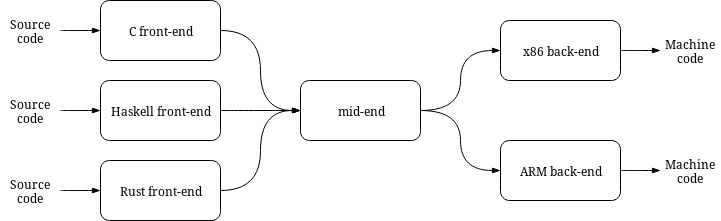
\includegraphics[width=12cm]{background/llvm/figures/three_phase_compiler}
	\caption{Three-phase compiler construction. The mid-end is somtimes called an \textit{optimizer}
	and the back-end a \textit{code generator}}
	\label{fig:three_phase_compiler}
\end{figure}

In the case of LLVM, the interface between the front-end and the mid-end is known as the
LLVM IR (\textit{Intermediate Representation}) and is a strongly typed, RISC-like virtual
instruction set that abstracts some details about the machine, such as function call
conventions and registers \cite[Section~11.3]{aosa-llvm}. To implement a programming language
one would then only have to implement a front-end, that is translate the source code to
LLVM IR. One could then pick and choose from the already existing LLVM optimizer passes
and LLVM back-end implementations to complete the compiler\cite[Section~11.5]{aosa-llvm}.

Only the back-end is of concern to this thesis, so it will focus exclusively on that.

\subsection{LLVM back-end}

A LLVM back-end, also known as a LLVM code generator, has a well defined input. The
LLVM IR\cite[Section~11.4.1]{aosa-llvm}. The output is often an object file, but a backend
can also act as an interpreter. For most of it's task, a LLVM backend uses what is called
the \textit{machine IR} to represent the code during the different stages.

The LLVM back-end is responsible for five main tasks: intruction selection, instruction
scheduling, register allocation, code layout optimization and assembly code emission
\cite{llvm-writing-backend, llvm-codegenerator-highlevel, aosa-llvm}. They are performed
mostly in isolation to each other \cite[Section~11.5]{aosa-llvm}, which simplifies the
architecture but introduces some interesting challenges.

The general behaviour of an LLVM back-end is that it transforms LLVM IR to machine code
for a specific target platform. Exactly what it produces depends on the target architecture
but it is common to generate assembly corresponding to the instruction set of the target
machine \cite[Section~11.5]{aosa-llvm}.

This paper does not cover instruction selection or other, smaller, back-end tasks such as
optimization, ABI implementation, exception handling etc \cite[at~1:47]{welcome-to-backend}.

\subsubsection{LLVM Machine Representation}

To represent machine specific IR LLVM uses what is called "Machine specific representation".
The machine specific representation consists of target agnostic, in-memory representations
of functions (MachineFuntion), basic blocks (MachineBasicBlock) and instructions
(MachinrInstr) \cite{llvm-mir-lang-ref, llvm-codegenerator-machinecode}.

The machine specific representation can be represented as the LLVM MIR (\textit{Machine
Intermediate Representation}), which is a human readable, YAML serialized format. It is
used to test code generation passes in LLVM. That is, we can stop the LLVM back-end
prematurely and view the current progress in the form of an LLVM MIR
\cite{llvm-mir-lang-ref}.

For example, the iterative factorial function written in C:

\lstinputlisting[language=C,tabsize=2,frame=single,breaklines=true,showstringspaces=false,
backgroundcolor= \color{lightgray}]
{background/llvm/examples/factorial.c}

gets translated to the following MIR when targeting the Hexagon V4 architecture and
terminating after instruction selection, right before register allocation and instruction
scheduling.

\lstinputlisting[tabsize=2,frame=single,breaklines=true,showstringspaces=false,
backgroundcolor= \color{lightgray}]
{background/llvm/examples/factorial.mir}

Courtesy of the Unison documentation for the code examples \cite{unison-docs-examples}.

What is interesting to note is that there is an infinite number of virtual registers available,
starting from \%0 and incrementing, as well as some abstract intructions, such as the PHI
function.

\subsubsection{Instruction Scheduling}
% https://llvm.org/docs/CodeGenerator.html#scheduling-and-formation
Instruction scheduling is the task of choosing how and in which order the selected instructions
will run. In the case of LLVM the scheduling phase is logically seperate from the selection
phase \cite{llvm-codegenerator-scheduling}. There exists a wide variety of architecture
and they all have different limitations and constraints.

A single issue processor is a processor that issues one instruction per cycle, and thus
logically easier to compile code for.

Today there exists multiple issue architectures in three major categories\cite[Section~3.7]{caqa},

\begin{itemize}
	\item Statically scheduled superscalar processors
	\item VLIW (Very Long Instruction Word) processors
	\item Dynamically scheduled superscalar processors
\end{itemize}

VLIW processors issues a fixed number of instructions every cycle as packages \cite[Section~3.7]{caqa},
or \textit{bundles} as the are called in LLVM \cite{llvm-codegenerator-bundles}. This
architecture has also been called EPIC (explicitly parallel instruction computer), which
make it clear that these require the parallelism between instruction to be explicitly
indicated statically, i.e. by the compiler \cite[Section~3.7]{caqa}.

The superscalar processors issue varying number of instructions per cycle and can be either
in-order (in the case of statically scheduled) and out-of-order (dynamically scheduled).
Dynamically scheduled superscalar processors exploits ILP during runtime and thus required
no compiler support \cite[Section~3.4]{caqa}, while statically schedules superscalar
processors requires the compiler to generate the entire execution schedule pre-execution
\cite[Section~3.7]{caqa}.

As previously mentioned LLVM is a set of libraries, and thus no one way to schedule instructions
in LLVM exists. However, the key factors to take into account during instruction scheduling
is generally to make use of architecture specific features (such as VLIW), avoiding pipeline
stalls by rearranging instructions \cite{Section~3.2]{caqa}, register pressure
\cite{llvm-inst-sched-superscalar-vliw} etc. When scheduling instructions the main
constraint is data-dependencies. Some instructions depends on the result of previous
instructions, and must thus be scheduled sequentially. In the cases where these
dependencies does not exists (or can be broken by e.g introducing new temporaries) the
instructions can be scheduled in a different order or in parallel (if the hardware allows it).

Instruction scheduling can be seen as a problem where the input is a list of resources
(e.g ALUs, FPUs, presence of VLIW) and a execution cycles for each instruction, and the
output is the instruction in the sequence they should be executed for optimal performance
(with regards to whatever factor you are optimizing for). In other words, maximize
\textit{instruction level parallellism} \cite{inst-sched-cmu}. Of course this problem is
very difficult.

\subsubsection{Register Allocation}

There are a few different problem concering register allocation, including (but not limied
to), coalescing, spilling move insertion and assigment \cite{alloc-deconstructed,
llvm-codegenerator-allocation}.

Coalescing is the attempt to eliminate move instructions that refers to identical locations,
i.e. remove unnecessary moves. When spilling a register you allocate the variable on the
stack to free up the register for another temporary ("spilling" the temporary to the stack)
and move insertion is used to split the lifetime of temporaries \cite{alloc-deconstructed}.

In general the task is modeled as a graph-coloring problem. The first step is then to
perform a \textit{liveliness analysis}, where you analyse the temporaries in the program
to determine which values has to co-exist (i.e. be placed in different registers). With
the liveliness analysis in hand a graph can be constructed where each node is a temporary,
edges represents that the two temporaries must be assigned to distinct registers and the
colors are registers. E.g for a machine with 64 registers you would use at most 64 colors
to color the graph. Assigning a temporary to a specific register (perhaps because of
calling conventions) would then be to "pre-color" the corresponding node. Coalescing in
this model would be to "merge" two nodes and spilling would be to remove a node. Spilling
is usually a consequence of not being able to find a coloring of the graph, thus
necessitating that a node be removed \cite{alloc-deconstructed}.

\subsubsection{Problems with LLVM Approach}
% http://i.stanford.edu/pub/cstr/reports/cs/tn/95/22/CS-TN-95-22.pdf
It is a common approach to treat instruction scheduling and register allocation as two
distinct steps in the back-end pipeline, and indeed so does LLVM \cite[Section~11.5]{aosa-llvm}.
There are two approaches to this, either you start with one or the other. Starting with
instruction scheduling is, nowadays, more common. Doing the register allocation first was
mainly used in the early days of compilers when machines didn't have as many registers
\cite[\pno~3]{combining-alloc-sched}.

% citation needed
% maybe here: https://pdfs.semanticscholar.org/5246/7f742a206b075324ec17b9b7f9d539f52ec8.pdf
% it mentions that it needs to be merged which is good.
Seperating these steps in such a manner leads to some problems, and usually some instruction
scheduling is once again performed after the register allocation \cite{welcome-to-backend}.
If a register needs to be spilled then the dependency graph which we based our schedule on is no longer valid. Re-doing
these steps is quite expensive though, as you would essentially throw out all previous
progress as soon as a register is spilled. Instead, modern compiler generate (potentially)
suboptimal code. Not very modern.

More subtle, machine specific problems can also occur even after both instruction scheduling
and register allocation has happened. When setting up stack frames and resolving frame
indices one might find oneself in the situation of needing both additional instructions
\textit{and} more registers. This can occur because of the targets limited number of immediates,
for examples we might be doing something like this:

\lstinputlisting[tabsize=2,frame=single,breaklines=true,showstringspaces=false,
backgroundcolor= \color{lightgray}]
{background/llvm/examples/initial_inst.mir}

Where we attempt to store a value given a (symbolic) frame index. This frame index will be replaced by
the LLVM Prolog Epilog Inserter to a stack pointer and an offset. For example it might
generate something like this:

\lstinputlisting[tabsize=2,frame=single,breaklines=true,showstringspaces=false,
backgroundcolor= \color{lightgray}]
{background/llvm/examples/stack_offset.mir}

where it has replaced the frame index with an offset of 4104 from the stack pointer. However,
if the target cannot encode 4104 directly as an immediate we need another instruction to
calculate this offset, and another register to store the offset in, like so:

\lstinputlisting[tabsize=2,frame=single,breaklines=true,showstringspaces=false,
backgroundcolor= \color{lightgray}]
{background/llvm/examples/temporary_resources.mir}

Thus, we are in a situation where we need more instructions and more register after both
instruction scheduling and register allocation is already over. LLVM solves this with something
they call \textit{register scavenging}, which is not something that will be covered here
\cite[at~48:53]{welcome-to-backend}.

While this specific example might have needed to incorporate instruction selection into
the mix as well, it is nonetheless a difficulty.

Instruction selection, instruction scheduling and register allocation are all tasks that
depend on each other, but in order to make them managable by current solution they need
to be performed mostly in isolation to each other. Combining instruction scheduling and
register allocation is a popular subject of research
\cite{constraint-based, combining-alloc-sched, integrated-sched-alloc-techniques}.
